\documentclass[a4paper,12pt]{article}
\usepackage[utf8]{inputenc}
\usepackage[spanish]{babel}
\usepackage{estilosbase}


\title{Suite informática de Teoría Algorítmica de Grafos}
\author{Alumno: Moisés Gautier Gómez\\Director: Antonio J. Tomeu Hardasmal}
\date{\today}


\begin{document}

\pagestyle{empty}
\begin{titlepage}

  \begin{center}

    
\includegraphics[scale=0.2]{logo_uca.png} \\

    \vspace{2.0cm}

    \LARGE{\textbf{ESCUELA SUPERIOR DE INGENIERÍA}} \\

    \vspace{1.0cm}

    \Large{\textbf{INGENIERÍA TÉCNICA EN INFORMÁTICA DE SISTEMAS}} \\

    \vspace{3.0cm}

    \Large{Suite informática de Teoría Algorítmica de Grafos} \\

    \vspace{2.0cm}

    \Large{Moisés Gautier Gómez} \\

  \end{center}
\end{titlepage}


\maketitle
\pagestyle{empty}
\abstract{\noindent El siguiente documento se presenta a modo de resumen que
  complementa la memoria del mismo Proyecto Fin de Carrera, entregado el
  día de la presentación de este proyecto. El proyecto que nos ocupa
  es una suite informática que trata sobre la teoría algorítmica de grafos y su representación mediante la herramienta Graphvisualx.}

\tableofcontents 

\cleardoublepage
\pagestyle{plain}
\section{Introducción}

Muchas de las aplicaciones computacionales, naturalmente, no implican sólo un conjunto de elementos o items, sino también un conjunto de conexiones de pares de dichos elementos o items. Las relaciones implícitas en estas conexiones nos plantean inmediatamente algunas preguntas: ¿Hay alguna forma de ir de un punto a otro siguiendo las conexiones realizadas? ¿Sobre cuantos elementos o items se puede navegar partiendo de uno del conjunto dado? ¿Cual es la forma más óptima de llegar desde un elemento a otro del conjunto?\\

La teoría de grafos, es una rama importante de las matemáticas combinatorias que se ha estudiado intensamente durante cientos de años. Muchas propiedades importantes y útiles de los grafos se han demostrado, sin embargo, otros muchos problemas de mucha complejidad (problemas de complejidad NP o irresolubles en tiempo polinómico) siguen sin resolverse.\\

Al igual que muchos de los dominios de otros problemas que se han estudiado, la investigación sobre teoría algorítmica de grafos es relativamente reciente. Aunque algunos de los algoritmos fundamentales son viejos, la mayoría de los más destacados han sido descubiertos en las últimas décadas. Incluso los algoritmos más simples de grafo son de utilidad en programas informáticos y los algoritmos no tan triviales son algunos de los más elegantes e interesantes jamás desarrollados.\\

Siempre será habitual el interés de saber cuál es el algoritmo más eficiente para resolver un problema que la propia resolución de este. El estudio de las características de rendimiento de los algoritmos de grafos es un reto porque:\\

\begin{itemize}
  
\item El coste de un algoritmo no sólo depende de las propiedades del conjunto de elementos o items, sino también en numerosas propiedades de las conexiones de dichos conjuntos (y las propiedades globales del grafo que se implican en dichas conexiones o uniones de elementos del conjunto).

\item Los modelos exactos de los tipos de grafos posibles que pueden aparecer son difíciles de desarrollar.

\end{itemize}

A menudo trabajaremos con los límites de coste del peor caso para los algoritmos de grafos, a pesar de que podrían representar estimaciones pesimistas sobre el desarrollo real en ciertas situaciones. Afortunadamente existen una serie de algoritmos que son óptimos e implican un pequeño uso de trabajo para su resolución. Habrá algoritmos que se podrán analizar con exactitud para situaciones específicas, pero cuando no fuera posible dicho análisis tan exacto, se tendrá que prestar especial atención a las propiedades de los distintos grafos que se podrán dar en situaciones reales o prácticas y evaluar como estas propiedades pueden afectar al rendimiento de los algoritmos.\\

Comenzaremos trabajando con las definiciones básicas y propiedades de los grafos, usando para ello una nomenclatura estándar para describir los contenidos. A continuación, se define el TAD (Tipo Abstracto de Datos) que será nuestra estructura de trabajo y forma de representación de los grafos computacionalmente independiente del lenguaje de programación o de alto nivel usado para su implementación. Las dos estructuras de datos más importantes para la representación de grafos son matriz de adyacencias o listas de adyacencias.\\

La elección entre las dos estructuras de datos depende principalmente de si el grafo de trabajo es denso o disperso, aunque como siempre, la naturaleza de las operaciones que se utilizarán juegan un papel importante en la decisión sobre cual estructura usar.\\

\subsection{Objetivos}

El objetivo principal del proyecto es elaborar una aplicación informática que sea capaz de representar un grafo y los posibles algoritmos de procesado que se pueden aplicar a los grafos.

La aplicación deberá cumplir los siguientes requisitos:

\begin{itemize}
\item Se mostrará en una primera instancia la representación del grafo una vez se haya introducido los valores asociados para las aristas o vértices.

\item Una vez seleccionado el algoritmo de procesamiento o la operación pertinente se mostrará el grafo origen y el resultado de la operación en la misma ventana para resaltar los cambios efectuados por el procesamiento del algoritmo.

\item Habrá un listado con los algoritmos más reseñables de la historia sobre teoría de grafos, así como una breve descripción de ellos y un ejemplo desarrollando la resolución que se dio para solventarlos. 

\end{itemize}

Es importante aclarar el dominio de conocimiento sobre los algoritmos de teoría de grafos que se han seleccionado. Los algoritmos tratados en este proyecto y su resultado en la aplicación pertenecen en su gran mayoría a temario desarrollado en las asignaturas de Matemáticas Discretas, Estructuras de Datos II y Análisis de Algoritmos I y II de la titulación de Ingeniero Técnico Informático de Sistemas de la Universidad de Cádiz.

El desarrollo del contenido teórico se realizará en un lenguaje sencillo y claro para permitir que un estudiante universitario de cualquier Ingeniería Informática puede comprender los contenidos matemáticos sin apenas dificultad añadida.

\subsection{Contexto: Historia sobre la teoría de grafos}

El primer artículo sobre teoría de grafos fue escrito por el famoso matemático suizo Euler, y apareció en 1736. Desde un punto de vista matemático, la teoría de grafos parecía, en sus comienzos, bastante insignificante, puesto que se ocupaba principalmente de pasatiempos y rompecabezas. Sin embargo, avances recientes en las matemáticas y, especialmente, en sus aplicaciones han impulsado en gran medida la teoría de grafos. Si ya en el siglo XIX se usaban los grafos en áreas como la teoría de circuitos eléctricos o los diagramas moleculares, hay en la actualidad parcelas de las matemáticas - la teoría de relaciones matemáticas, por ejemplo - en las que los grafos son una herramienta natural; además, han surgido muchas aplicaciones a cuestiones de carácter práctico: emparejamientos, problemas de transporte, flujo en redes y lo que, en general, se engloba bajo el nombre de "programación". La teoría de grafos ha hecho acto de presencia en campos tan dispares como la economía, la psicología o la biología, y todo ello sin renunciar a los pasatiempos, en especial si incluimos entres ellos al famoso problema de los cuatro colores, que intriga hoy a los matemáticos tanto como el primer día.\\

Dentro de las matemáticas, la teoría de grafos se considera una rama de la topología; no obstante, también está muy relacionada con el álgebra y la teoría de matrices.\\

Los grafos de intervalos aparecen al tratar una amplía variedad de problemas. \\

Arqueología. Numerosos arqueólogos han utilizado grafos de intervalos al tratar de ordenar ciertos acontecimientos de manera cronológica. En un experimento, un grupo de arqueólogos investigó los objetos encontrados en un gran número de tumbas, con la intención de ordenarlas cronológicamente. Partiendo de la base de que si dos utensilios diferentes aparecían juntos en una misma tumba, entonces sus períodos de tiempo debían solaparse, los arqueólogos construyeron un grafo en el que los vértices correspondían a los objetos, y las aristas a los pares de objetos hallados juntos en una misma tumba. Representando este grafo como un grafo de intervalos, e interpretando cada intervalo como un período de tiempo durante el cual se usó el artefacto, pudieron finalmente ordenar las tumbas cronológicamente.\\

Análisis literario. También se han usado grafos de intervalos a la hora de investigar la posible autoría de obras literarias discutidas, tales como ciertas obras de Platón. Se estudia la aparición de diversos rasgos del estilo de un autor (como el uso del ritmo) en varias obras literarias. Dibujando un grafo en el que los vértices corresponden a dichos rasgos literarios, y las aristas a los pares de rasgos que aparecen juntos en una misma obra, llegamos a una situación muy similar a la de nuestro ejemplo arqueológico. Como antes, podemos entonces investigar si el grafo resultante puede representarse como un grafo de intervalos, lo que abre la posibilidad de ordenar las obras cronológicamente. Esta forma de proceder ha permitido, en ocasiones, relacionar el estilo de la obra literaria en disputa con el estilo del autor en cuestión, determinando así la probable autoría.\\

Genética. Los grafos de intervalos aparecieron originalmente al estudiar un problema de genética más concretamente, el de determinar si la fina estructura en el interior del gen está dispuesta o no de manera lineal. Al analizar la estructura genética de un virus en concreto, el genetista Seymour Benzer consideró las mutaciones cuyos segmentos extraviados se solapan, por lo que dibujó un grafo en el que los vértices correspondían a las mutaciones, y las aristas a los pares de mutaciones cuyos segmentos perdidos se solapaban. Representando este grafo como grafo de intervalos, pudo mostrar que (para ese virus) la evidencia en favor de una disposición lineal dentro del gen era aplastante.\\

\subsection{Alcance}

El proyecto Suite informática de Teoría Algorítmica de Grafos dará como resultado la aplicación Graphvisualx que cumplirá con todos los objetivos y especificaciones indicados en el apartado anterior.\\

La aplicación Graphvisualx se distinguirá en varias partes: el contenido teórico de cada algoritmo a desarrollar como posible comprensión del desarrollo del mismo, el desarrollo de los algoritmos con una entrada ya sea bien en formato fichero o introducida desde la entrada de estándar en el momento de ejecución de la aplicación y contenidos bibliográficos haciendo incapie en algoritmos clásicos de la materia y su resolución desarrollada.\\

Todo lo que se encuentra desplegado en la aplicación viene descrito en notación formal matemática (algoritmos descritos bajo código fuente de la aplicación) describiendo su análisis coste temporal y algunos ejemplos al uso. (Tener en cuenta que el usuario tiene ciertas nociones básicas sobre lo que es un grafo, sus posibles representaciones y operaciones básicas de conjuntos).\\

\subsection{Visión global}

En cuanto a la estructura de esta Memoria del Proyecto de Fin de Carrera, tras este capítulo donde se presentan los objetivos y la visión en general del proyecto, se expone el desarrollo de las definiciones básicas de un grafo así como la mayoría de términos relacionados con él.\\

El capítulo siguiente contiene la descripción general de todos los algoritmos desarrollados para esta aplicación en una notación formal matemática y mediante algunos ejemplos de uso del algoritmo según unos valores de entrada aleatorios. \\

Seguidamente describiremos algunos de los algoritmos clásicos más destacados que ha dado la historia de la teoría algorítmica de grafos así como las posibles soluciones que sus autores dieron en su día para dichos problemas. Además se incluirá otro capítulo en donde tendrá especial relevancia el concepto de notación asintótica y NP-Complejidad. \\

Finalmente, se presentan las conclusiones generales obtenidas una vez realizado el proyecto para pasar inmediatamente a los manuales de usuario y de instalación. \\

Además se presentan las referencias bibliográficas donde se incluyen las fuentes consultadas para la elaboración de este proyecto, un resumen que engloba las generalidades fundamentales de la aplicación, una guía de utilización (manual de usuario), una guía de instalación, un compendio del software utilizado para el desarrollo y otro de los lenguajes de programación, el desarrollo del calendario mediante un diagrama de Gantt describiendo con detalle las distintas etapas de desarrollo del proyecto y finalmente la licencia completa del documento. \\

\subsection{Software utilizado}

En la realización de este proyecto se ha empleado el lenguaje de programación Java (J2ME) en su versión 1.6, empleando además la utilidad de openJDK para dicha plataforma Java.\\

Para la realización y estructuración del proyecto se ha empleado la herramienta IDE NetBeans v. 7.0.\\

La documentación y las figuras expuestas en este documento y derivados se han creado mediante el lenguaje de interpretación \LaTeX\ y para las figura el paquete de opciones de tikz.\\

\subsubsection{Licencia}

La aplicación gráfica Graphvisualx es software libre: usted puede redistribuirlo y / o modificar bajo los términos de la Licencia Pública General de GNU según lo publicado por la Free Software Foundation, ya sea la versión 3 de la Licencia, o (a su elección) cualquier versión posterior.\\

Este programa se distribuye con la esperanza de que sea útil, pero SIN NINGUNA GARANTÍA, incluso sin la garantía implícita de COMERCIALIZACIÓN o IDONEIDAD PARA UN PROPÓSITO PARTICULAR. Ver el GNU General Public License para más detalles.\\

Debería haber recibido una copia de la Licencia Pública General de GNU junto con este programa. Si no es así, consulte \href{http://www.gnu.org/licenses/}{GNU Licenses}.\\

\section{Conceptos básicos}

\subsection{Generalidad}

Definiremos un grafo como un sistema matemático abstracto. No obstante, para desarrollar el conocimiento de los mismos de forma intuitiva los representaremos mediante diagramas. A estos diagramas les daremos también el nombre de grafos, aun cuando los términos y definiciones no estén limitados únicamente a los grafos que pueden representarse mediante diagramas.

Un grafo es un conjunto de puntos y un conjunto de líneas donde cada línea une un punto con otro. 

\subsection{Definición formal}

\begin{fondo}
Llamaremos grafo, G, al par ordenado formado por un conjunto finito no vacío, V, y un conjunto, A, de pares no ordenados de elementos del mismo.\\
\smallskip
\quad V es el conjunto de los vértices o nodos del grafo.\\
\smallskip
\quad A será el conjunto de las aristas o arcos del grafo.\\
\smallskip
Utilizaremos la notación G = (V,A) para designar al grafo cuyos conjuntos de vértices y aristas son, respectivamente, V y A.
\end{fondo}

A cualquier arista de un grafo se le puede asociar una pareja de vértices del mismo. Si $u$ y $v$ son dos vértices de un grafo y la arista $a$ esta asociada con este par, escribiremos $a = uv$.\\

Por ejemplo, si\\
\[ V = \{v_1, v_2, v_3, v_4, v_5\} \]
y\\
\[ A = \{v_1v_2, v_1v_3, v_1v_4, v_2v_4, v_2v_5\} \]
entonces el grafo $G = (V,A)$ tiene a $v_1, v_2, v_3, v_4$ y $v_5$ como vértices y sus aristas son $v_1v_2, v_1v_3, v_1v_4, v_2v_4$ y $v_2v_5$.

Se definirán los conceptos de vértices adyacentes e incidentes además de los tipos de grafos posibles y sus posibles representaciones mediante matrices de adyacencia/incidencia o listas de adyacencia. También se definirán concepto como conectividad de grafos, puntos de corte y puentes.

\subsection{Disperso frente a Denso}

Se define la densidad de un grafo como el promedio del grado de los vértices, o $2 A \setminus V$. Un grafo \emph{denso} es un grafo cuyo promedio de grado de vértices es proporcional a $V$; por otro lado un grafo disperso es un grafo cuyo complementario es denso. En otras palabras, consideramos que un grafo es denso si $A$ es proporcional a $V^2$ sino será disperso. Esta definición asintótica no es necesariamente significativa para un grafo en particular, pero la distinción es clara en general: Un grafo que cuenta con miles de vértices y miles de decenas de aristas es claramente disperso, y un grafo que tiene cientos de vértices y millones de aristas es claramente denso. Podríamos contemplar un grafo disperso con miles de millones de vértices, pero un grafo denso con miles de millones de vértices tendrá un numero abrumador de aristas. \\

Saber si un grafo es disperso o denso, es generalmente un factor clave en la selección de un algoritmo eficiente para procesar el grafo. Por ejemplo, para un problema en concreto, podríamos desarrollar un algoritmo que tomara alrededor de $V^2$ y otro que tomara alrededor de $A \lg A$ pasos. Estas fórmulas nos dicen que el segundo algoritmo sería mejor para grafos dispersos, mientras que el primero sería preferible para grafos densos. Por ejemplo, un grafo denso con millones de aristas podría tener sólo unos miles de vértices: en este caso $V^2$ y $A$ serían comparables en valor, y el algoritmo de $V^2$ pasos sería 20 veces más rápido que el algoritmo de $A \lg A$ pasos. Por otro lado, un grafo disperso con millones de aristas también tendría millones de vértices, por lo que el algoritmo de $A \lg A$ pasos podría ser millones de veces más rápido que el algoritmo de $V^2$ pasos. Podríamos hacer concesiones específicas sobre la base del análisis de estas fórmulas con más detalle, pero por lo general es suficiente en la práctica usar los términos disperso y denso de manera informal para ayudarnos a comprender las características fundamentales de rendimiento.\\

\section{Algoritmos}

Se analizarán en profundidad todos los algoritmos tratados en el proyecto de fin de carrera intentando en la medida de lo posible una fácil comprensión para el lector falto de conocimientos básicos y para el que tenga unas nociones mayores sobre la materia. Los algoritmos a tratar serán muy variados:
\begin{itemize}
\item Caminos y Ciclos de Euler.
\item Caminos y Ciclos de Hamilton.
\item Grafos ponderados.
\begin{itemize}
\item Caminos más cortos desde un vértice:Dijkstra.
\item Caminos más cortos:Floyd.
\item Existencia de caminos:Warshall.
\item Árboles de expansión mínimos:Kruskal.
\item Árboles de expansión mínimos:Prim.
\end{itemize}
\item Búsqueda en grafos: en profundidad (Depth First Search).
\item Búsqueda en grafos: en anchura (Breadth First Search).
\item Vértice coloración: número cromático.
\item Ordenación Topológica.
\end{itemize}

\figuratikz{1}{Un grafo dirigido ponderado y los pasos que realiza el algoritmo de Dijkstra en el grafo. En cada paso se colorean los nuevos vértices y las nuevas aristas procesadas.}
{
  \tikzstyle{place}=[circle,thick,draw=blue!20,fill=green!20,minimum size=5mm]
  \tikzstyle{texto}=[]
  \tikzstyle{process}=[circle,thick,draw=blue!20,fill=red!20,minimum size=5mm]

  \begin{scope}


    \node [place] (c1) {$v_5$};

    \node [process] (c2) [right of=c1,xshift=.5cm,yshift=2cm] {$v_1$}
    edge [post] node [above,xshift=-.2cm] {$1$} (c1);

    \node [place] (c3) [right of=c1,xshift=2cm] {$v_2$}
    edge [pre] node [above,xshift=.2cm] {$7$} (c2);

    \node [place] (c4) [below of=c1,xshift=.4cm,yshift=-.6cm] {$v_4$}
    edge [pre] node [below,yshift=.2cm,xshift=-.3cm] {$1$} (c1) 
    edge [pre] node [above,xshift=.3cm] {$6$} (c2)
    edge [post]  node [above] {$3$} (c3);

    \node [place] (c5) [below of=c3,xshift=-.4cm,yshift=-.6cm]  {$v_3$}
    edge [pre] node [above,xshift=-.3cm] {$4$} (c2)
    edge [post] node [below] {$5$} (c4)
    edge [post] node [below,yshift=.1cm,xshift=.3cm] {$2$} (c3) ;

    \node [process] (d1) [right of=c3,xshift=.2cm] {$v_5$};

    \node [process] (d2) [right of=d1,xshift=.5cm,yshift=2cm] {$v_1$}
    edge [red,post] node [above,xshift=-.2cm] {\textcolor{black}{$1$}} (d1);

    \node [place] (d3) [right of=d1,xshift=2cm] {$v_2$}
    edge [pre] node [above,xshift=.2cm] {$7$} (d2);

    \node [place] (d4) [below of=d1,xshift=.4cm,yshift=-.6cm] {$v_4$}
    edge [pre] node [below,yshift=.2cm,xshift=-.3cm] {$1$} (d1) 
    edge [pre] node [above,xshift=.3cm] {$6$} (d2)
    edge [post]  node [above] {$3$} (d3);

    \node [place] (d5) [below of=d3,xshift=-.4cm,yshift=-.6cm]  {$v_3$}
    edge [pre] node [above,xshift=-.3cm] {$4$} (d2)
    edge [post] node [below] {$5$} (d4)
    edge [post] node [below,yshift=.1cm,xshift=.3cm] {$2$} (d3) ;


    \node [process] (e1) [right of=d3,xshift=.2cm] {$v_5$};

    \node [process] (e2) [right of=e1,xshift=.5cm,yshift=2cm] {$v_1$}
    edge [red,post] node [above,xshift=-.2cm] {\textcolor{black}{$1$}} (e1);

    \node [place] (e3) [right of=e1,xshift=2cm] {$v_2$}
    edge [pre] node [above,xshift=.2cm] {$7$} (e2);

    \node [process] (e4) [below of=e1,xshift=.4cm,yshift=-.6cm] {$v_4$}
    edge [red,pre] node [below,yshift=.2cm,xshift=-.3cm] {\textcolor{black}{$1$}} (e1) 
    edge [pre] node [above,xshift=.3cm] {$6$} (e2)
    edge [post]  node [above] {$3$} (e3);

    \node [place] (e5) [below of=e3,xshift=-.4cm,yshift=-.6cm]  {$v_3$}
    edge [pre] node [above,xshift=-.3cm] {$4$} (e2)
    edge [post] node [below] {$5$} (e4)
    edge [post] node [below,yshift=.1cm,xshift=.3cm] {$2$} (e3) ;

    \node [process] (f1) [below of=c1,yshift=-3.5cm,xshift=2cm] {$v_5$};

    \node [process] (f2) [right of=f1,xshift=.5cm,yshift=2cm] {$v_1$}
    edge [red,post] node [above,xshift=-.2cm] {\textcolor{black}{$1$}} (f1);

    \node [place] (f3) [right of=f1,xshift=2cm] {$v_2$}
    edge [pre] node [above,xshift=.2cm] {$7$} (f2);

    \node [process] (f4) [below of=f1,xshift=.4cm,yshift=-.6cm] {$v_4$}
    edge [red,pre] node [below,yshift=.2cm,xshift=-.3cm] {\textcolor{black}{$1$}} (f1) 
    edge [pre] node [above,xshift=.3cm] {$6$} (f2)
    edge [post]  node [above] {$3$} (f3);

    \node [process] (f5) [below of=f3,xshift=-.4cm,yshift=-.6cm]  {$v_3$}
    edge [red,pre] node [above,xshift=-.3cm] {\textcolor{black}{$4$}} (f2)
    edge [post] node [below] {$5$} (f4)
    edge [post] node [below,yshift=.1cm,xshift=.3cm] {$2$} (f3) ;

    \node [process] (g1) [below of=d3,yshift=-3.5cm,xshift=-.8cm] {$v_5$};

    \node [process] (g2) [right of=g1,xshift=.5cm,yshift=2cm] {$v_1$}
    edge [red,post] node [above,xshift=-.2cm] {\textcolor{black}{$1$}} (g1);

    \node [process] (g3) [right of=g1,xshift=2cm] {$v_2$}
    edge [pre] node [above,xshift=.2cm] {$7$} (g2);

    \node [process] (g4) [below of=g1,xshift=.4cm,yshift=-.6cm] {$v_4$}
    edge [red,pre] node [below,yshift=.2cm,xshift=-.3cm] {\textcolor{black}{$1$}} (g1) 
    edge [pre] node [above,xshift=.3cm] {$6$} (g2)
    edge [red,post]  node [above] {\textcolor{black}{$3$}} (g3);

    \node [process] (g5) [below of=g3,xshift=-.4cm,yshift=-.6cm]  {$v_3$}
    edge [red,pre] node [above,xshift=-.3cm] {\textcolor{black}{$4$}} (g2)
    edge [post] node [below] {$5$} (g4)
    edge [post] node [below,yshift=.1cm,xshift=.3cm] {$2$} (g3) ;
    
\end{scope}  

}

\section{La complejidad algorítmica}

Cuando tenemos que resolver un problema, es posible que estén disponibles varios algoritmos adecuados. Evidentemente, desearíamos seleccionar el mejor. Esto plantea la pregunta de cómo decidir entre varios algoritmos cuál es preferible. Si solamente tenemos que resolver uno o dos casos pequeños de un problema más bien sencillo, quizá no nos importe demasiado qué algoritmo utilizaremos: en este caso podríamos decidirnos a seleccionar sencillamente el que sea más fácil de programar, o uno para el cual ya exista un programa, sin preocuparnos por sus propiedades teóricas. Sin embargo, si tenemos que resolver muchos casos, o si el problema es difícil, quizá tengamos que seleccionar de forma más cuidadosa.\\

El enfoque \emph{empírico} (o a posteriori) para seleccionar un algoritmo consiste en programar las técnicas competidoras e ir probándolas en distintos casos con ayuda de una computadora. El enfoque \emph{teórico} (a priori) que es el que casi siempre se toma como referencia, consiste en determinar matemáticamente la cantidad de recursos necesarios para cada uno de los algoritmos \emph{como función del tamaño de los casos considerados}. Los recursos que más nos interesan son el tiempo de computación y el espacio de almacenamiento, siendo el primero normalmente el más importante. \\

El \emph{tamaño} de un ejemplar se corresponde formalmente con el número de \emph{bits} que se necesitan para representar el ejemplar en una computadora, utilizando algún esquema de codificación precisamente definido y razonablemente compacto. Sin embargo, para hacer más claros nuestros análisis, lo normal será que seamos menos formales, y utilizaremos la palabra ``tamaño'' para indicar cualquier entero que mida de alguna forma el número de componentes de un ejemplar. Por ejemplo, cuando estamos hablando acerca de ordenaciones, mediremos normalmente el tamaño de un ejemplar por el número de items que hay que ordenar ignorando el hecho consistente en que cada uno de estos items ocuparía más de un bit para representarlo en una computadora. De manera similar, cuando hablemos acerca de grafos, mediremos normalmente el tamaño de un ejemplar por el número de nodos o de aristas (o de ambos) implicados. Apartándonos un poco de esta regla general, sin embargo, cuando hablemos acerca de problemas que impliquen enteros, daremos algunas veces la eficiencia de nuestros algoritmos en términos del \emph{valor} del ejemplar que estemos considerando, en lugar de considerar su tamaño (que sería el número de bits \emph{bits} necesarios para representar en binario este valor).\\

La ventaja de la aproximación teórica es que no depende ni de la computadora que se esté utilizando, ni del lenguaje de programación, ni siquiera de las habilidades del programador. Se ahorra tanto el tiempo que se habría invertido innecesariamente para programar un algoritmo ineficiente, como el tiempo de máquina que se habría desperdiciado comprobándolo. Lo que es más significativo, se nos permite estudiar la eficiencia del algoritmo cuando se utiliza en casos de todos los tamaños. Esto no suele suceder con la aproximación empírica, en la cual las consideraciones prácticas podrían obligarnos a comprobar los algoritmos sólo en un pequeño número de ejemplares arbitrariamente seleccionados y de tamaño moderado. Dado que suele suceder que los algoritmos recién descubiertos empiezan a comportarse mejor que sus predecesores sólo cuando ambos se utilizan en ejemplares grandes, este último punto resulta especialmente importante. \\

Si deseamos medir la cantidad de espacio que utiliza un algoritmo en función del tamaño de los ejemplares, está a nuestra disposición una unidad natural, a saber, el \emph{bit}. Independientemente de la máquina que se esté utilizando, la noción de un \emph{bit} de almacenamiento está bien definida. Si, por otra parte, tal como suele suceder, deseamos medir la eficiencia de un algoritmo, en términos del tiempo que se necesita para llegar a una respuesta, entonces no existe una opción tan evidente. Está claro que no se puede pensar en expresar esta eficiencia, digamos, en segundos, puesto que no se dispone de una computadora estándar a la cual se pudieran referir todas las medidas (existe una computadora estándar, pero es un modelo teórico: la maquina de Turing).\\

Una respuesta a este problema es la que viene dada por el \emph{principio de invariancia}, que afirma que dos implementaciones distintas de un mismo algoritmo no diferirán en su eficiencia en más de alguna constante multiplicativa. Si esta constante fuera, por ejemplo, cinco, entonces sabemos que si la primera implementación requiere un segundo para resolver casos de un cierto tamaño, entonces la segunda implementación (quizá en una máquina distinta, o escrita en un lenguaje de programación distinto) no requerirá más de 5 segundos para resolver los mismos casos. Para ser más exactos, si dos implementaciones del mismo algoritmo necesitan $t_1(n)$ y $t_2(n)$ segundos, respectivamente, para resolver un caso de tamaño $n$, entonces siempre existen constantes positivas $c$ y $d$ tales que $t_1(n) \leq ct_2(n)$ y $t_2(n) \leq dt_1(n)$ siempre que $n$ sea lo suficientemente grande. En otras palabras, el tiempo de ejecución de cualquiera de las implementaciones está acotado por un múltiplo constante del tiempo de ejecución de la otra; la decisión de a qué implementación llamaremos primera, y a cuál llamaremos segunda, es irrelevante. La condición de que $n$ sea suficientemente grande no es realmente necesaria, según la \textbf{regla del umbral}:\\

\begin{fondo}
Una función $t_n$ pertenece al orden de $f(n):\ O(f(n))$
\begin{itemize}
\item cuando está acotada superiormente por $f(n)$ para valores de $n$ suficientemente grandes y
\item haciendo abstracción de posibles constantes multiplicativas
\end{itemize}
\begin{center}
\[O(f(n)) = \Bigl\{ t: \mathbb{N} \rightarrow \mathbb{R}^{\geq 0} \Bigl| \exists\ c \in \mathbb{R}^{+} , \exists n_{0} \in \mathbb{N} \Bigl| \forall n \geq n_{0} : t(n) \leq c \cdot f(n) \Bigl\} \]
\end{center}

\end{fondo}

Sin embargo, al incluirla suele ser posible hallar constantes más pequeñas $c$ y $d$ que las que se hallarían en caso contrario. Esto resulta útil si estamos intentando calcular buenas cotas acerca del tiempo de ejecución de una implementación cuando conocemos el tiempo de ejecución de la otra.\\

Volviendo a la cuestión de la unidad que se debe utilizar para expresar la eficiencia teórica de un algoritmo, el principio de invariancia nos permite decidir que no va a existir tal unidad. En su lugar, expresaremos solamente el tiempo requerido por el algoritmo salvo una constante multiplicativa. Diremos que un algoritmo para algún problema requiere un tiempo del orden de $t(n)$ para una función dada $t$, si existe una constante positiva $c$ y una implementación del algoritmo capaz de resolver todos los casos de tamaño $n$ en un tiempo que no sea superior a $ct(n)$ segundos. \\

El uso de segundos en esta definición es evidentemente arbitrario: sólo se necesita modificar la constante para acotar el tiempo por $at(n)$ años o por $bt(n)$ microsegundos. Por el principio de invariancia, si cualquier implementación del algoritmo tiene la propiedad requerida, entonces también la tienen todas las demás, aunque la constante multiplicativa pueda cambiar de una implementación a otra.\\

\subsection{Notación Asintótica}

Esta notación se denomina ``asintótica'' porque trata acerca del comportamiento de funciones en el límite, esto es, para valores suficientemente grandes de su parámetro. En consecuencia, los argumentos basados en la notación asintótica pueden no llegar a tener un valor práctico cuando el parámetro adopta valores ``de la vida real''. Sin embargo, en las enseñanzas de la notación asintótica suelen tener una relevancia significativa. Esto se debe a que, un algoritmo que sea superior asintóticamente suele ser (aunque no siempre) preferible incluso en casos de tamaño moderado.\\

\subsubsection{La $O$ mayúscula}

Sea $t: \mathbb{N} \rightarrow \mathbb{R}^{\geq 0}$ una función arbitraria de los números naturales en los números reales no negativos, tal como $t(n) = 5n^2 + \frac{100}{3}n + 2$. Se suele pensar que $n$ representa el tamaño del ejemplar sobre el cual es preciso que se aplique un algoritmo dado, y en $t(n)$ como representante de la cantidad de un recurso dado que se invierte en ese ejemplar por una implementación particular de este algoritmo. Por ejemplo, podría ser que la implementación invirtiera $t(n)$ microsegundos en el ejemplar peor en un caso de tamaño $n$, o quizá $t(n)$ represente la cantidad de espacio. Tal como se ha visto, la función $t(n)$ puede muy bien depender de la implementación más que depender únicamente del algoritmo. Recuerde sin embargo el principio de invariancia, que dice que la \emph{razón} de los tiempos de ejecución de dos implementaciones diferentes del mismo algoritmo siempre está acotada por encima y por debajo mediante constantes predeterminadas. (Las constantes pueden depender de las implementaciones pero no del tamaño del ejemplar).\\

Considérese ahora una función $f: \\mathbb{N} \rightarrow \mathbb{R}^{\geq 0}$ tal como $f(n) = n^2$. Diremos que $t(n)$ está en el \emph{orden de f(n)} si $t(n)$ está acotada superiormente por un múltiplo real positivo de $f(n)$ para todo $n$ suficientemente grande. Matemáticamente, esto significa que existe una constante real y positiva $c$ y un entero umbral $n_0$ tal que $t(n) \leq cf(n)$, siempre que $n \geq n_0$.\\

Por ejemplo, considérese las funciones $f(n)$ y $t(n)$ definidas anteriormente. Está claro que tanto $n \leq n^2$ como $1 \leq n^2$, siempre que $n \geq 1$. Por tanto, siempre y cuando $n \geq 1$:

\begin{center}
\[ t(n) = 5n^2 + \frac{100}{3}n + 2 \]
\[ \geq 5n^2 + \frac{100}{3}n^2 + 2n^2 \]
\[ = 40n^2 = 40 f(n) \]
\end{center}

Tomando $c = 40$ (o cualquier valor mayor) y $n_0 = 1$, concluiremos por tanto que $t(n)$ es del orden de $f(n)$ por cuanto $t(n) \leq cf(n)$ siempre que $n \geq n_0$. Por tanto es conveniente disponer de un símbolo matemático para representar \emph{el orden de}. Una vez más sea $f: \mathbb{N} \rightarrow \mathbb{R}^{\geq 0}$ una función arbitraria de los números naturales en los reales no negativos. Le indicará mediante $O(f(n))$ - que se lee ``$O$ de $f(n)$'' - \emph{el conjunto} de todas las funciones $t: \mathbb{N} \rightarrow \mathbb{R}^{\geq 0}$ tales que $t(n) \leq cf(n)$ para todo $n \geq n_0$ para una constante positiva real $c$ y para un umbral entero $n_0$. En otras palabras:
\begin{center}
\[ O(f(n)) = \big\{ t: \mathbb{N} \rightarrow \mathbb{R}^{\geq 0} \big| \exists c \in \mathbb{R}^+\ \exists n_0 \in \mathbb{N}\ \forall n \geq n_0\ [t(n) \leq cf(n)] \big\} \]\\
\end{center}

\begin{nota}
A partir de ahora la notación del término $O(f(n))$ será $O(f)$ empleada en otros libros o referencias para facilitar su uso al lector. Igualmente la notación para la función $f(n)$ se sustituirá con la notación simple de $f$ siempre que no haya confusión.\\
\end{nota}

La notación $O(f)$, denota al conjunto de las funciones de $t$ que crecen a lo más tan rápido como $f$, es decir, las funciones $t$ tales que, mediante una \emph{constante multiplicativa}, $f$ llega a ser en algún momento una cota superior para $t$. Así pues la correspondencia con la definición es intuitiva: el cuantificador existencial sobre $c$ formaliza la expresión \emph{constantes multiplicativas}, y $n_0$ indica a partir de qué punto $f$ es realmente una cota superior para $t$.\\

A modo de ejemplo, aplicando la definición puede comprobarse que para $f(n) = n^2$ y $t(n) = n$ se tiene que $t \in O(f))$ pero sin embargo $f \notin O(t)$. Para $f(n) = 3n^2$ y $t(n) = 100n^2$ se tiene que $t \in O(f)$ y $f \in O(t)$.\\

La notación $O(f)$ tiene las siguientes propiedades, cualesquiera que sean las funciones $f,t$ y $g$.\\
\begin{enumerate}
\item \emph{Invariancia multiplicativa}. Para toda constante $c \in \mathbb{R}^+$,
\[ t \in O(f) \iff c \cdot t \in O(f) \]
Se demuestra por simple aplicación de la definición.
\item \emph{Reflexividad}. $f \in O(f)$. Basta comprobar la definición.
\item \emph{Transitividad}. Si $g \in O(t)$ y $t \in O(f)$ entonces $g \in O(f)$. Se demuestra mediante sencillas manipulaciones aritméticas.
\item \emph{Criterio de caracterización}. $t \in O(f) \iff O(t) \subseteq O(f)$. Se deduce fácilmente de las dos anteriores.
\item \emph{Regla de la suma para $O$}. $O(f+t) = O(max(f,t))$, donde denotamos $f+t$ la función que sobre el argumento $n$ vale $f(n)+t(n)$, y $max(f,t)$ la función sobre la que el argumento $n$ vale el máximo de $\{f(n),t(n)\}$. Frecuentemente esta regla se aplica así: si $t_1 \in O(f_1)$ y $t_2 \in O(f_2)$, entonces $t_1 + t_2 \in O(max(f_1,f_2))$.
\item \emph{Regla del producto para $O$}. Si $t_1 \in O(f_1)$ y $t_2 \in O(f_2)$, entonces $t_1 \cdot t_2 \in O(f_1 \cdot f_2)$, donde denotamos $f \cdot t$ la función que sobre el argumento $n$ vale $f(n) \cdot t(n)$.
\item \emph{Invariancia aditiva}. Para toda constante $c \in \mathbb{R}^{+}$,
\[ t \in O(f) \iff c + t \in O(f) \]
En consecuencia inmediata de la regla de la suma.
\end{enumerate}

\section{Conclusiones}

Durante la realización de la aplicación \emph{Graphvisualx: Suite informática de Teoría Algorítmica de Grafos} como trabajo de fin de carrera, he conseguido profundizar mi conocimiento sobre este mundo matemático y sus posibilidades de aplicaciones en la vida cotidiana cuya utilización va más allá de lo que cabría pensar. Además he profundizado en el conocimientos sobre la complejidad algorítmica y sus problemas importantes como son la Indecibilidad y la Intratabilidad. También he aprendido a manejar un nuevo lenguaje de programación, en este caso Java, dado que en la titulación hay muy pocas asignaturas en las cuales se imparta porque se sustituye por el lenguaje C y C++ en su mayoría. Dicho hecho ha ocasionado más de un retraso a la hora de realizar las implementaciones de los algoritmos y estructuras de datos, debido a la falta de práctica con este lenguaje como se comenta anteriormente.\\

Una vez terminado este proyecto se espera haber cumplido con los objetivos propuestos:
\begin{itemize}
\item Se mostrará en una primera instancia la representación del grafo una vez se haya introducido los valores asociados para las aristas o vértices.

\item Una vez seleccionado el algoritmo de procesamiento o la operación pertinente se mostrará el grafo origen y el resultado de la operación en la misma ventana para resaltar los cambios efectuados por el procesamiento del algoritmo.

\item Habrá un listado con los algoritmos más reseñables de la historia sobre teoría de grafos, así como una breve descripción de ellos y un ejemplo desarrollando la resolución que se dio para solventarlos. 

\end{itemize}

Ha sido un largo y tedioso trabajo durante los últimos 6 meses que será liberado de forma oficial bajo licencia libre una vez presentado el proyecto ante un tribunal para su evaluación. Este hito supondrá la culminación de esta primera etapa de proyecto, a partir de la cuál podrá ser leído y trabajado por aquel que lo considere interesante. La siguiente etapa sería la de revisión, mejora y ampliación del contenido.\\

\subsection{Expectativas de futuro}

El producto obtenido de este proyecto de fin de carrera es un producto final. Por su naturaleza está ideado en principio para la trata y uso de los posibles algoritmos implementados en un principio, dado que no se facilita ningún soporte directo para la implementación de un mayor contenido algorítmico debido a ausencia del mismo o recientes descubrimientos de nuevas teorías algorítmicas.\\

Se podrían implementar algoritmos de teoría de grafos sobre redes de comunicaciones o relaciones de ontología de la web que dado a la falta de conocimientos en la materia se han obviado para una posible actualización futura.\\


\section{Organización temporal}

Para la elaboración de este proyecto de fin de carrera me ha sido necesario estudiar de nuevo el funcionamiento de muchos algoritmos sobre grafos que, previamente estudiados durante la titulación, había obviado en ciertos matices que habían que aclara para acometer con precisión una implementación fina y eficiente.\\ Además, la falta de práctica con el lenguaje de programación Java también ha puesto de su parte para la demora de muchos puntos del proyecto.\\

Dicha organización temporal se reparte en tareas que iba cumpliendo a medida que iba desarrollando el software Graphvisualx, explicando durante las jornadas de trabajo los hitos conseguidos y los problemas que habían surgido durante el desarrollo de la misma.

\vfill
\pagebreak
\begin{figure}[H]
\begin{center}
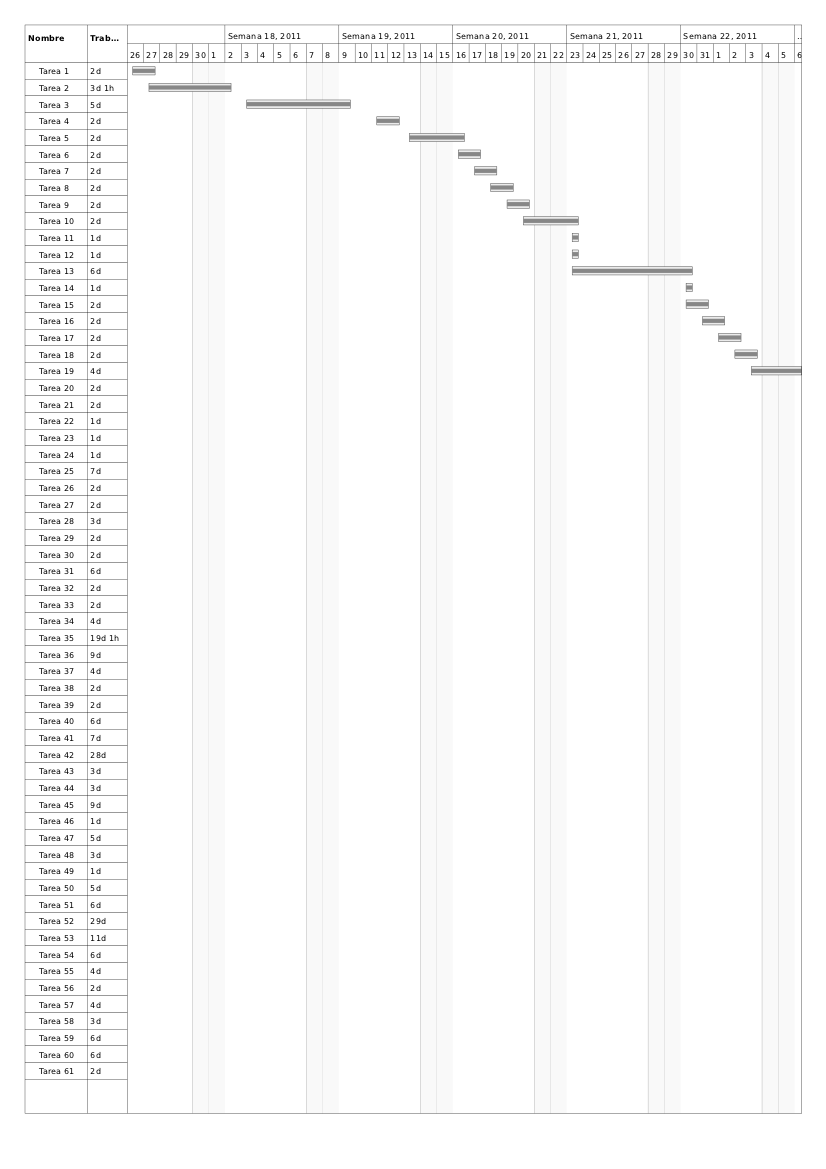
\includegraphics[width=16.5cm]{planificacion_graphvisualx_1.png}
\caption{Planificación Temporal del proyecto - Desde el 26 de Abril de 2011.}
\end{center}
\end{figure}

\pagebreak
\begin{figure}[H]
\begin{center}
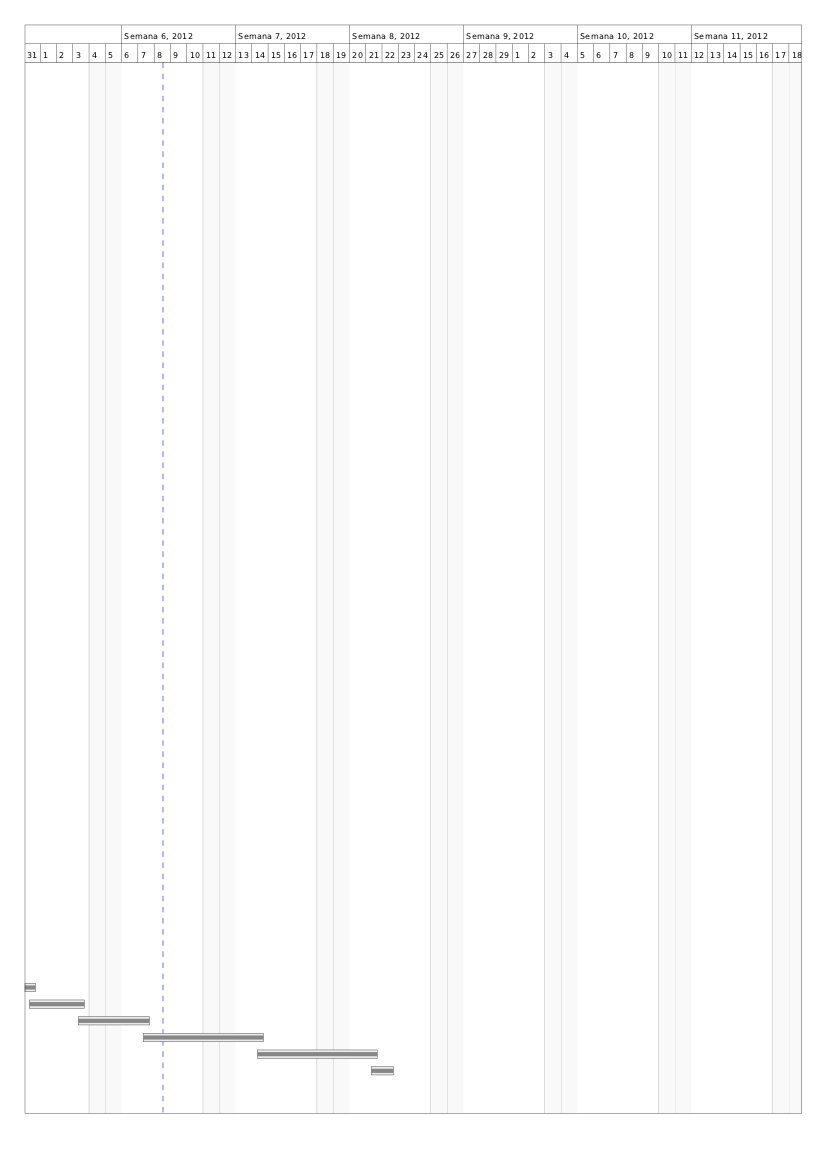
\includegraphics[width=16.5cm]{planificacion_graphvisualx_7.png}
\caption{Planificación Temporal del proyecto - Desde el 30 de Enero 2012.}
\end{center}
\end{figure}

\pagebreak
\begin{figure}[H]
\begin{center}
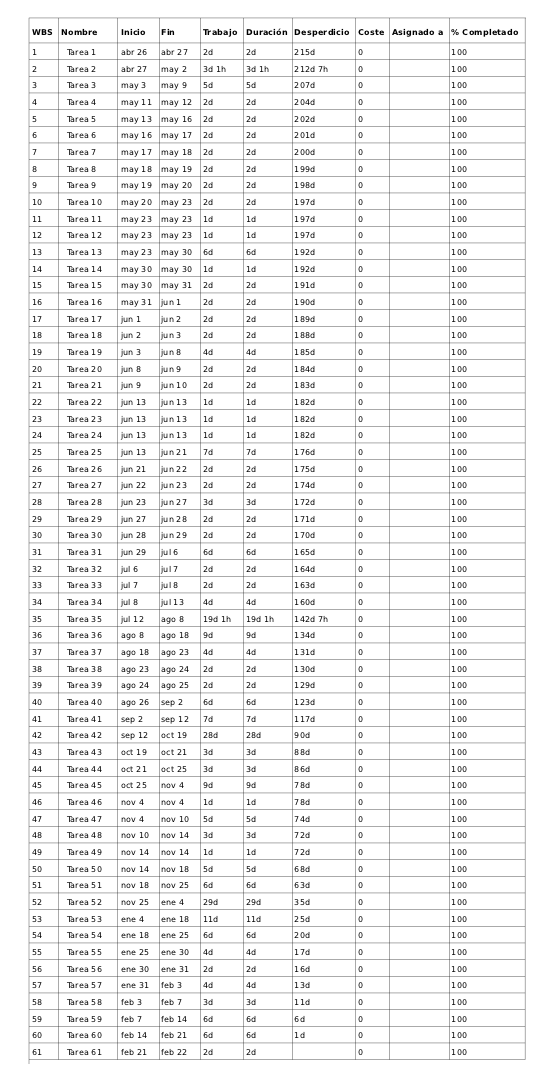
\includegraphics[width=11.5cm]{planificacion_graphvisualx_8.png}
\caption{Planificación Temporal del proyecto.}
\end{center}
\end{figure}


\section{Guía de usuario}

\subsection{Interfaz gráfica}

Una interfaz gráfica de usuario (GUI) presenta un mecanismo amigable al usuario para interactuar con una aplicación. Una GUI proporciona a una aplicación una ``apariencia visual'' única. Al proporcionar distintas aplicaciones en las que los componentes de la interfaz de usuario sean consistentes e intuitivos, los usuarios pueden familiarizarse en cierto modo con una aplicación, de manera que pueden aprender a utilizarla en menor tiempo y con mayor productividad.\\

Las GUIs se crean a partir de componentes de la GUI. A éstos se les conoce también como controladores o widgets (accesorios de ventana) en otros lenguajes. Un componente de la GUI es un objeto con el cual interactúa el usuario mediante el ratón, el teclado u otra forma de entrada, como el reconocimiento de voz.\\

\begin{figure}[H]
\begin{center}
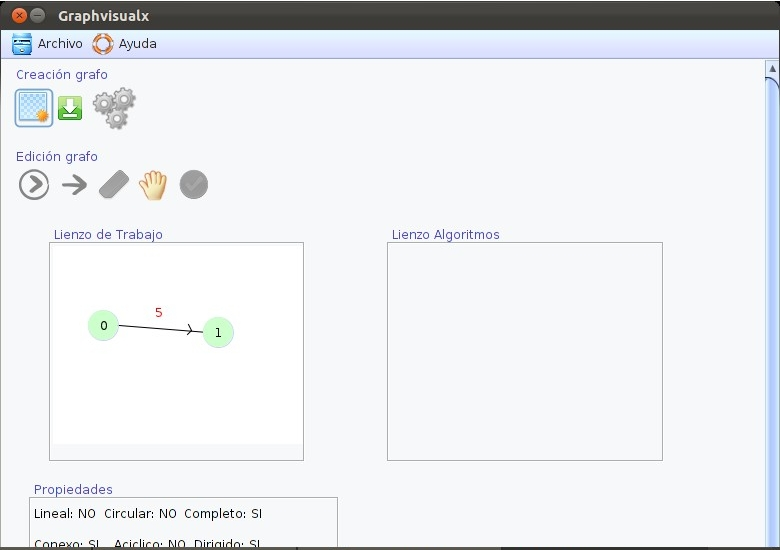
\includegraphics[width=14cm]{./imagenes_documentacion/Graphvisualx_31_1_2012/captura_4.jpeg}
\caption{Captura final de la aplicación Graphvisualx.}
\end{center}
\end{figure} 

\clearpage
\nocite{*}
\bibliographystyle{plain}
\bibliography{biblio}
\pagestyle{empty}

\end{document}